%-----------------------------------------------------------------------------%
\chapter{\babTiga}
%-----------------------------------------------------------------------------%

Pada bab ini dijelaskan mengenai tahapan, rancangan \& implementasi sistem, pengumpulan \& pengolahan data dan teknik evaluasi yang digunakan pada penelitian ini.

%-----------------------------------------------------------------------------%
\section{Tahapan Penelitian}
%-----------------------------------------------------------------------------%

\lipsum[1-2]

%-----------------------------------------------------------------------------%
\section{Rancangan dan Implementasi Sistem}
%-----------------------------------------------------------------------------%

As shown in the flowchart Figure \ref{fig_program_flowchart}, our system is composed of four main components: \textbf{NLP pipeline}, \textbf{triple candidate generator}, \textbf{triple selector} and \textbf{token expander}. Each of them are explained further in following subsections.

\begin{figure}
\centering
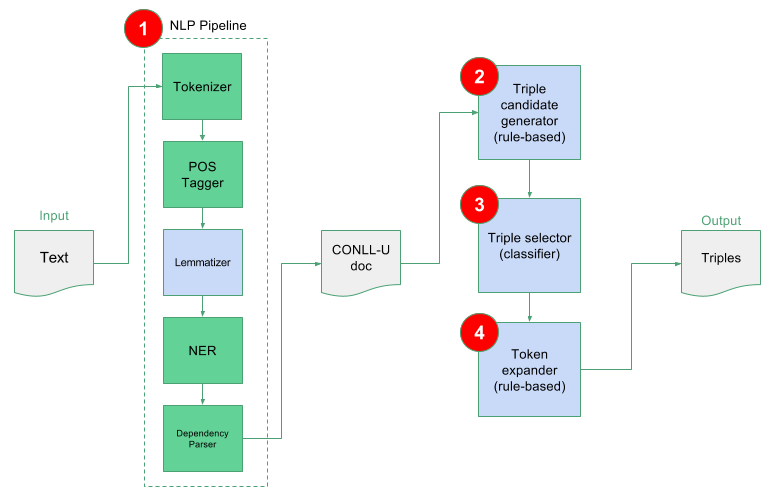
\includegraphics[width=\textwidth]{../images/program_flowchart.png}
\caption{Indonesian open domain information extraction flowchart}
\label{fig_program_flowchart}
\end{figure}

\subsection{NLP Pipeline}

The NLP pipeline is a series of NLP tasks that annotates one or more sentences and saves them in CONLL-U\footnote{CONLL-U format description \url{http://universaldependencies.org/format.html}} format, a token-based sentence annotation format containing lemma, POS tag, dependency relation and a slot for additional annotation. The pipeline assumes that each sentence in the input document is separated by new line so preprocessing may be required. The detail of each model the pipeline are described below:

\begin{enumerate}

\item Tokenizer \\
We use default tokenizer provided by Stanford Core NLP, \verb|PTBTokenizer| \citep{manningptbtokenizer}, which mimics Penn Treebank 3 tokenizer\footnote{Penn Treebank 3 \url{https://catalog.ldc.upenn.edu/LDC99T42}}. While this tokenizer provides many options to modify its behavior, we stick to default configuration that split sentence by whitelines to get the tokens.\\

\item Part of Speech Tagger \\
We trained default Stanford Core NLP \verb|MaxentTagger| \citep{toutanova2003feature} with Indonesian universal POS tag dataset which we convert from dependency parsing dataset\footnote{UD Indonesian dataset \url{https://github.com/UniversalDependencies/UD_Indonesian}}. This POS tagger uses Max Entropy (multi-class logistic regression) classifier which yields \textbf{93.68\%} token accuracy and \textbf{63.91\%} sentence accuracy when trained using 5,036 sentences and tested with 559 sentences from the dataset. \\

\item Lemmatizer \\
The lemmatizer used in this pipeline, \verb|IndonesianLemmaAnnotator|, is implemented based on an existing Indonesian rule-based Lemmatizer \citep{suhartono2014lemmatization} with some improvements:

\begin{itemize}
\item Reimplementation in Java language
\item Usage of in-memory database to speed up dictionary lookup
\item Integration with Stanford Core NLP annotator API for reusability
\end{itemize}

This lemmatizer yields \textbf{99\%} accuracy when tested using dataset of 5,638 token-lemma pairs\footnote{Indonesian Lemmatizer \url{https://github.com/davidchristiandy/lemmatizer}}. We use lemma as one of the features for NER classifier. \\

\item Named-Entity Recognizer (NER)

Stanford NLP \verb|CRFClassifier| \citep{finkel2005incorporating}, a linear chain Conditional Random Field (CRF) sequence models, is trained using a dataset containing 3,535 Indonesian sentences with 5 entity class: Person, Organization, Location, Quantity and Time. When tested using 426 sentences, this models achieves 0.86 precision, 0.85 recall and \textbf{0.86} F1-score. The dataset itself is a combination between dataset from Faculty of Computer Science, University of Indonesia and a public dataset\footnote{Indonesian NER \url{https://github.com/yusufsyaifudin/indonesia-ner}}. \\

\item Dependency Parser

We relied on Stanford NLP \verb|nndep.DependencyParser| \citep{chen2014fast}, to annotate dependency relation of each token in the sentence. We train this transition-based neural network model using a Indonesian universal dependencies dataset of 5,036 sentences and 3,093 Indonesian word embedding\footnote{Indonesian word embedding \url{https://github.com/yohanesgultom/id-openie/blob/master/data/parser-id.embed}} (vector representation of words). Tested with 559 sentences, this model scores \textbf{70\%} UAS (Unlabeled Attachment Score) and \textbf{46\%} LAS (Labeled Attachment Score).

\end{enumerate}

The output of the pipeline is a CONLL-U document containing annotated sentence such as Figure \ref{fig_conllu_example}. The document becomes an input for next model, the triple candidate generator which is described in Section \ref{Triple Candidates Generator}. Since the annotations that are directly used by following process are POS tag, named entity and dependency relation, we estimate that the accuracy of this NLP pipeline is \textbf{65.30\%} which comes from the average of POS tagger sentence accuracy, NER F1-score (in percent) and dependency parser LAS. Additionally, this pipeline is built by extending Stanford Core NLP classes and packaged as single Java program (JAR) to improve reusability.

\begin{figure}
\centering
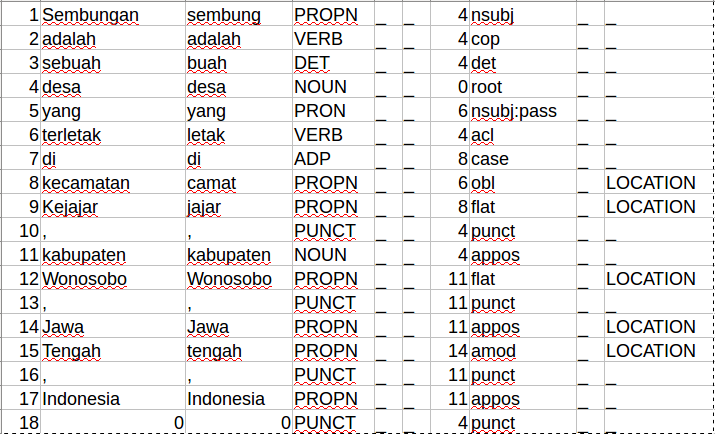
\includegraphics[scale=0.35]{../images/conllu_example.png}
\caption{Example of CONLL-U sentence annotation format}
\label{fig_conllu_example}
\end{figure}

\subsection{Triple Candidates Generator} \label{Triple Candidates Generator}

% Similar to TextRunner Self-Supervised Learner but doesn't automatically label triples

Triple candidates generator is used to extract relation triples candidates from CONLL-U document produced by NLP pipeline. It uses a set of rules listed in Table \ref{table_triple_candidate_generation_rules} to extract relations (predicates) and arguments (subjects and predicates) from the sentence. The results of triples extraction are not always the positive or valid relation triples so, unlike TextRunner \citep{banko2007open}, we cannot use them directly as training data for triple selector/classifier.

For example, applying the rules to an annotated sentence in Figure \ref{fig_conllu_example} will generate these 17 triples candidates where only five of them are valid triples (check-marked):

\begin{itemize}
\item (Sembungan, adalah, desa) \ding{51}
\item (Sembungan, adalah, terletak)
\item (Sembungan, adalah, kecamatan)
\item (Sembungan, adalah, kabupaten)
\item (Sembungan, adalah, Jawa)
\item (Sembungan, adalah, Tengah)
\item (Sembungan, adalah, Indonesia)
\item (Sembungan, terletak, kecamatan) \ding{51}
\item (Sembungan, terletak, kabupaten) \ding{51}
\item (Sembungan, terletak, Jawa) \ding{51}
\item (Sembungan, terletak, Tengah)
\item (Sembungan, terletak, Indonesia) \ding{51}
\item (desa, terletak, kecamatan)
\item (desa, terletak, kabupaten)
\item (desa, terletak, Jawa)
\item (desa, terletak, Tengah)
\item (desa, terletak, Indonesia)
\end{itemize}

In order to build a training data for the triple selector, we used triple candidates generator to generate 1,611 triple candidates from 42 sentences. As part of the label step, we manually label \textbf{132 positive} and \textbf{1,479 negative} triples which we use to train binary classifier as triple selector in the learn step.

During the extraction step, triple candidates generator is used in the system to extract unlabeled candidates from CONLL-U document. These unlabeled triples will be labeled by trained triple selector as described in  (referring to flowchart in Figure \ref{fig_program_flowchart}).

% Triple candidate generation rules
\begin{table}[!t]
\renewcommand{\arraystretch}{1.5}
\caption{Triple candidate generation rules}
\label{table_triple_candidate_generation_rules}
\centering
\begin{tabular}{l p{6cm}}
\hline
\textbf{Type} & \textbf{Condition} \\
\hline
Subject & Token's POS tag is either PROPN, NOUN, PRON or VERB \\
\space & Token is not "yang" nor "adalah" \\
\space & Token's dependency is neither "compound" nor "name" \\
\space & Token's dependency is either "compound" or "name" but separated by more than 2 tokens from its head \\
\hline
Predicate & Token's position is after Subject \\
\space & Token's POS tag is either VERB or AUX \\
\hline
Object & Token's position is after Subject and Predicate \\
\space & Token's POS tag is either PROPN, NOUN, PRON or VERB \\
\space & Token is not "yang" nor "adalah" \\
\space & Token's dependency is neither "compound" nor "name" \\
\space & Token's dependency is either "compound" or "name" but separated by more than 2 tokens from its head \\
\end{tabular}
\end{table}


\subsection{Triple Selector}  \label{Triple Selector}

Triple selector is a machine learning classifier trained using manually labeled dataset of valid and invalid relation triples. For example, given the input of 17 candidates in Section \ref{Triple Candidates Generator}, the selector will label the five check-marked triples as true and label the rest as false.

We use Random Forest \citep{breiman2001random}, an ensemble methods that aggregate classification results from multiple decision trees, as the model for the classifier. We use the Scikit-Learn\footnote{scikit-learn: machine learning in Python \url{http://scikit-learn.org}} implementation of Random Forest with following configuration:

\begin{itemize}
\item Decision tree criterion: Gini Impurity
\item Minimum number of samples to split tree node: 5 samples
\item Maximum features used in each tree: 4 (square root of the number of features)
\item Maximum trees depth: 8
\item Number of trees: 20
\item Class weight: balanced (prediction probability is multiplied by the ratio of training samples)
\end{itemize}

We discover the configuration by using Grid Search \citep{wasserman2015grid}, an exhaustive search algorithm to find optimal hyper-parameters, to find the best F1 score for Random Forest classifier using dataset described in Section \ref{Triple Candidates Generator}. 

We extract 17 features described in Table \ref{table_models_features} from each triple candidates. These features are based on POS tag, named-entity and dependency relation, instead of shallow syntactic features used by TextRunner or ReVerb \citep{banko2007open} \citep{etzioni2011open}. Every nominal features are also encoded and normalized along with the whole dataset by removing the mean and scaling to unit variance in order to improve the precision and recall of the classifier.

\begin{table}[!t]
\renewcommand{\arraystretch}{1.5}
\caption{Triple selector features}
\label{table_models_features}
\centering
\begin{tabular}{r l}
\hline
\textbf{\#} & \textbf{Triple Features} \\
\hline
1 & Subject token's POS tag \\
2 & Subject token's dependency relation \\
3 & Subject token's head POS tag \\
4 & Subject token's named entity \\
5 & Subject token's distance from predicate \\
6 & Subject token's dependency with predicate \\
7 & Predicate token's POS tag \\
8 & Predicate token's dependency relation \\
9 & Predicate token's head POS tag \\
10 & Predicate token's dependents count \\
11 & Object token's POS tag \\
12 & Object token's dependency relation \\
13 & Object token's head POS tag \\
14 & Object token's named entity \\
15 & Object token's dependents count \\
16 & Object token's distance from predicate \\
17 & Object token's dependency with predicate \\
\end{tabular}
\end{table}

During the train step, we use the dataset to train triple selector and save the best model as binary file. This model is included in the system to be use during the extraction step.

\subsection{Token Expander}

Instead of using lightweight noun phrase chunker \citep{banko2007open}, our system uses rule-based token expander to extract relation or argument clauses. While having different objective and approach, this token expander works similarly to Clause Selector in Stanford Open IE \citep{angeli2015leveraging} where the algorithm starts from a token then decides whether to expand to its dependents. Instead of using machine learning model like Clause Selector, it uses simple heuristics based on syntactical features (POS tag, dependency relation and named-entity) described in Table \ref{table_token_expansion_rules_s_o} and Table \ref{table_token_expansion_rules_p} to determine whether to: (1) expand a token to its dependent, (2) ignore the dependent or (3) remove the token itself. For example, token expander will expand check-marked triples in Section \ref{Triple Candidates Generator} into:

\begin{itemize}
\item (Sembungan, adalah, desa)
\item (Sembungan, terletak di, kecamatan Kejajar)
\item (Sembungan, terletak di, kabupaten Wonosobo)
\item (Sembungan, terletak di, Jawa Tengah)
\item (Sembungan, terletak di, Indonesia)
\end{itemize}

% Token expansion rules for Subject or Object token
\begin{table}[!t]
\renewcommand{\arraystretch}{1.5}
\caption{Token expansion rules for Subject or Object token}
\label{table_token_expansion_rules_s_o}
\centering
\begin{tabular}{r p{6cm} l}
\hline
\textbf{\#} & \textbf{Condition for Subject or Object Token} & \textbf{Action} \\
\hline
1 & If dependent's relation to the token  is either “compound”, “name”  or “amod” & Expand \\
2 & If dependent has same named entity as the token & Expand \\
3 & If dependent and the token are wrapped by quotes or double quotes  & Expand \\
4 & If the head is a sentence root & Ignore \\
5 & If dependent's POS tag is CONJ or its form is either “,” (comma) or “/” (slash) & Ignore \\
6 & If dependent's POS tag is either “VERB” or “ADP” & Ignore \\
7 & If dependent has at least one dependent with “ADP” POS tag & Ignore \\
8 & If the first or last token in expansion result has “CONJ” or “ADP” POS tag & Remove \\
9 & If the first or last index of expansion result is an incomplete parentheses symbol & Remove \\
10 & If the last index of expansion result is “yang” & Remove \\
11 & Else & Ignore \\
\hline
\end{tabular}
\end{table}

\begin{table}[!t]
\renewcommand{\arraystretch}{1.5}
\caption{Token expansion rules for Predicate token}
\label{table_token_expansion_rules_p}
\centering
\begin{tabular}{r p{6cm} l}
\hline
\textbf{\#} & \textbf{Condition for Predicate Token} & \textbf{Action} \\
\hline
1 & If dependent is “tidak” & Expand \\
2 & Else & Ignore \\
\hline
\end{tabular}
\end{table}

During the label step, token expander is used to make manual annotation process easier. We label a triple candidate as valid only if it makes sense after being expanded to clause. For example, \textit{(Sembungan, terletak, kecamatan)} doesn't seem to make sense before expanded to \textit{(Sembungan, terletak di, kecamatan Kejajar)}.